\documentclass[crop,border=0pt]{standalone}

\usepackage{mathtools}
\usepackage{tikz}
\usetikzlibrary{shapes,positioning,scopes,arrows}
\begin{document}
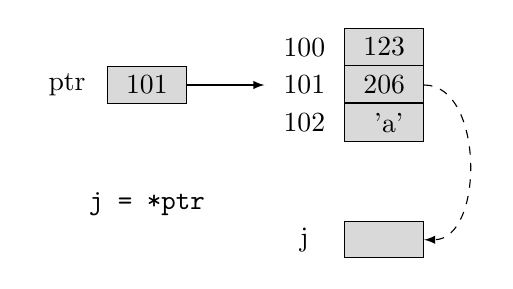
\begin{tikzpicture}[every node/.style={draw,align=center,text centered,minimum width=1cm}]

  {[every node/.append style={fill=gray!30}]
    \node (ptr) {101};
    \node [shape=rectangle split, rectangle split parts=3,
           minimum height=1.2em,
           text centered,right=2cm of ptr] (mem)
           {\nodepart{one}123 \nodepart{two} 206 \nodepart{three}\ 'a'};
    \node [below=of mem] (j) {\phantom{206}};
  }

  {[every node/.append style={draw=none}]
    \node [anchor=east] at (ptr.west) {ptr};
    \node [shape=rectangle split, rectangle split parts=3,
           minimum height=1.2em,
           text centered,anchor=east] (addr) at (mem.west)
           {\nodepart{one}100 \nodepart{two} 101 \nodepart{three}102};
    \node [anchor=east] at (j.west) {j};
    \node [below=1cm of ptr] {\texttt{j = *ptr}};
  }

  {[-latex]
    \draw (ptr) -- (addr.two west);
    \draw [dashed] (mem) edge [out=0, in=0] (j.east);
  }

\end{tikzpicture}
\end{document}
